% begin module trig-functions-graphs
\begin{frame}
\frametitle{Graphs of the Trigonometric Functions}
\begin{tabular}{cc}
\begin{tabular}{c}
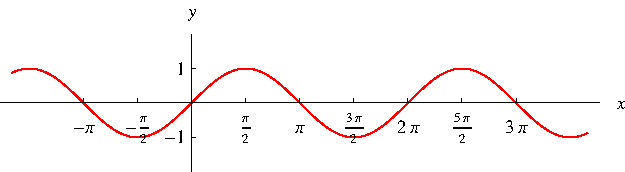
\includegraphics[width=8cm]{trigonometry/pictures/app-d-sin.pdf}%
\end{tabular}
& $y = \sin x$\\
\begin{tabular}{c}
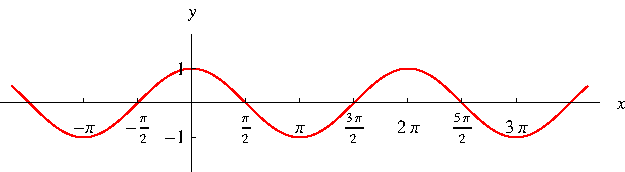
\includegraphics[width=8cm]{trigonometry/pictures/app-d-cos.pdf}%
\end{tabular}
& $y = \cos x$
\end{tabular}
\begin{itemize}
\item<2->  $\sin x$ has zeroes at $n\pi$ for all integers $n$.
\item<3->  $\cos x$ has zeroes at $\pi /2 + n\pi$ for all integers $n$.
\item<4->  $-1 \leq \sin x \leq 1$. 
\item<5->  $-1 \leq \cos x \leq 1$. 
\end{itemize}
\end{frame}


\begin{frame}
\begin{tabular}{cc}
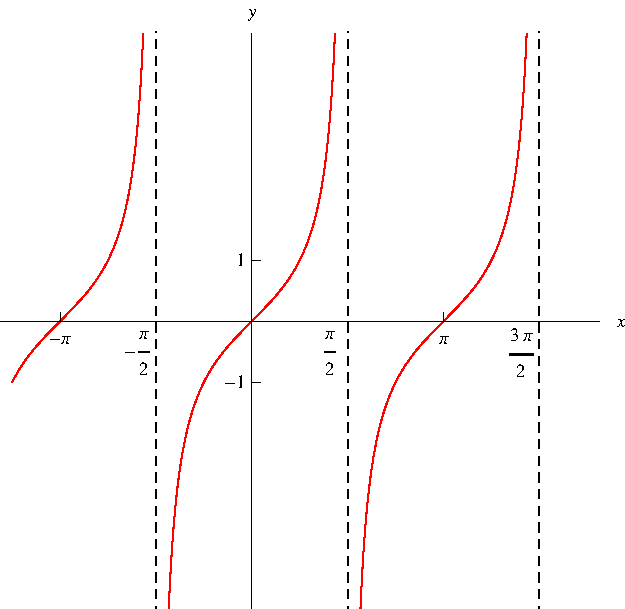
\includegraphics[width=5.5cm]{trigonometry/pictures/app-d-tan.pdf}%
&%
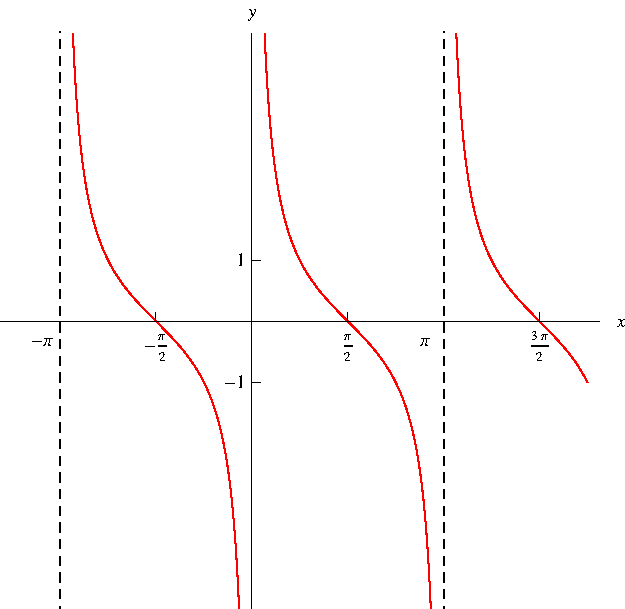
\includegraphics[width=5.5cm]{trigonometry/pictures/app-d-cot.pdf}%
\\%
$y = \tan x$ & $y = \cot x$\\
\end{tabular}
\end{frame}


\begin{frame}
\begin{tabular}{cc}
\only<handout:0| -1>{%
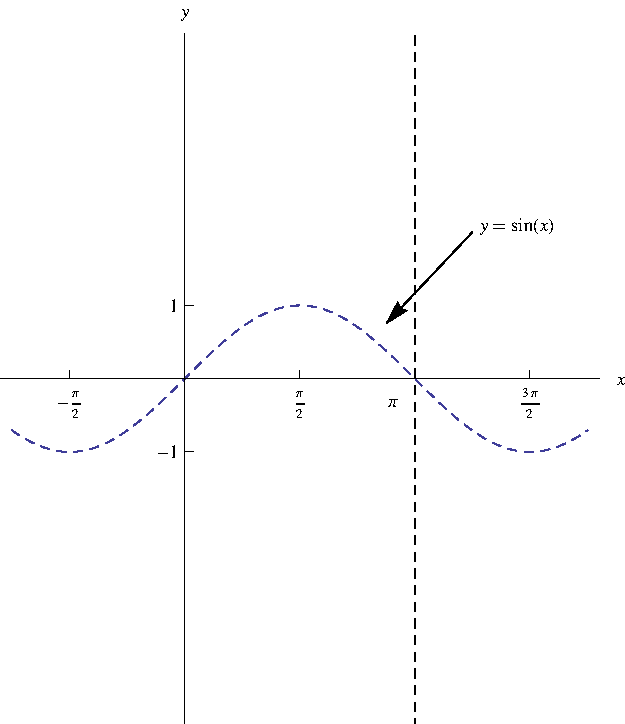
\includegraphics[width=5.5cm]{trigonometry/pictures/app-d-csca.pdf}%
}%
\only<2->{%
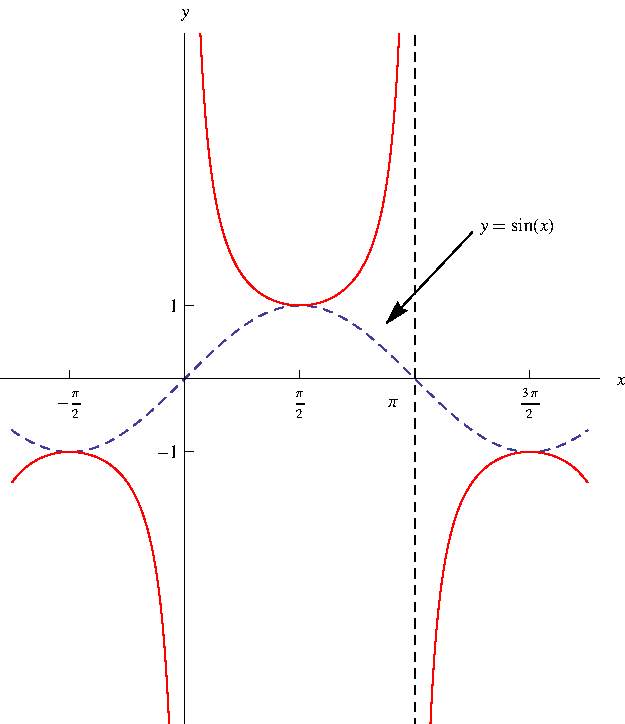
\includegraphics[width=5.5cm]{trigonometry/pictures/app-d-cscb.pdf}%
}%
&%
\only<handout:0| -2>{%
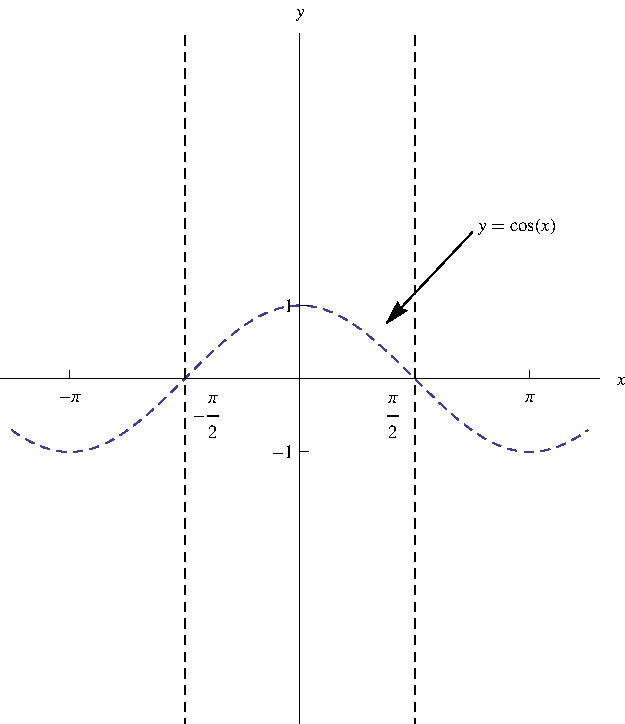
\includegraphics[width=5.5cm]{trigonometry/pictures/app-d-seca.pdf}%
}%
\only<3->{%
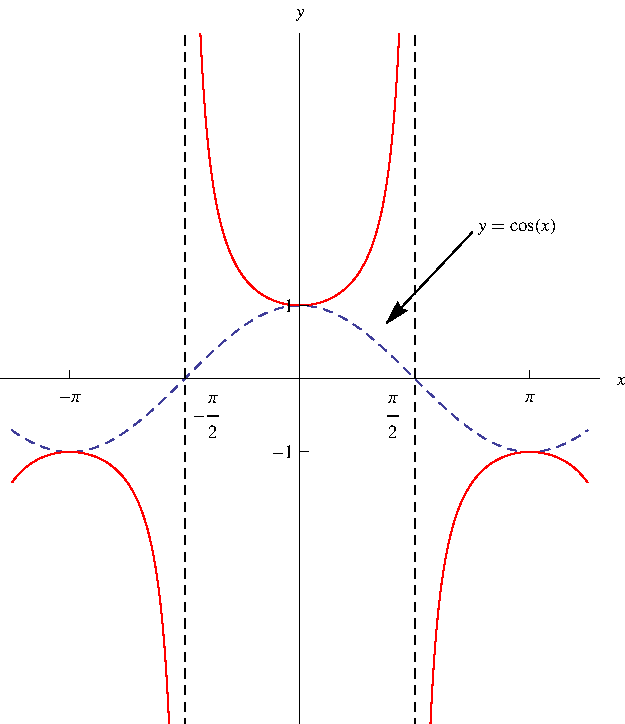
\includegraphics[width=5.5cm]{trigonometry/pictures/app-d-secb.pdf}%
}%
\\%
$y = \csc x$ & $y = \sec x$\\
\end{tabular}
\end{frame}
% end module trig-functions-graphs
